\chapter{Motor Learning in Virtual Reality}
\label{chapter:theoretical_background}
This chapter provides the theoretical background of Virtual Reality, Motor Learning, Visual Perspectives, handling physical load and injury risk metrics in a condensed form. For a more detailed description of these topics, please refere to the preceeding seminar thesis~\cite{seminarThesis} which is also digitally attached to this master's thesis. These topics are the most important aspects that serve as the foundation for this master's thesis. Subsequent, an analysis of related work is provided. This chapter gives insights into how this work is informed and differentiated from other researchers. Finally, the research contributoin statement is provided.

\section{Virtual Reality}
\label{section:mixed_reality}
Milgram and Kishinho~\cite{mrcontinuum} describe Mixed Reality (MR) for visual displays on a continuum. Virtual Reality (VR) is purely digital, and thereby the environment is blocked entirely. In Augmented Reality, the environment is visible and augmented with digital elements. During Motor Learning, the visual perception of the own body is desirable, because it is the most exact representation of the own body. Thereby, the approach of augmenting the real-world body with a virtual guidance visualisation (GV) is promising. However, today's AR-technology provides a small field of view. A solution to this could be the video see-through technology, but it is limited by latency and distortion~\cite{max}.\\
The body's perception can also be achieved by tracking the learner's body and render it over the learner's physical body. Though, the visual perception of the learner's body can be established in VR. Consequentially, this work will focus on Motor Learning in Virtual Reality.

\section{Motor Learning}
\label{section:motor_learning}
Motor Learning is achieved through instruction, trying, imitation or a combination of them~\cite{mlbook}. The process of Motor Learning can be divided into three parts: cognitive stage, associative stage and autonomous stage (ibid.). In the cognitive stage, training methods are most efficient, and the performance gain ist the highest among the stages (ibid.). Tasks that belong to this stage are thereby best suited for a study.\\
Movements can be classified by two means: by the \textit{particular movements} and based on the \textit{perceptual attributes} (ibid.). Based on the \textit{particular movements}, the classification is described by a continuum, compare figure~\ref{fig:movement_classification} left. On the extremes of the continuum are discrete movements and continuous movements. Between these extremes, serial movements are located. Discrete movements are too short for an evaluation. Continuous movements do not have a recognisable beginning, and thereby they are not suitable for the study in question either. Serial movements are chained discrete movements with a recognisable beginning and end. This allows a task decomposition and an evaluation of particular sub-tasks. Furthermore, serial movements are generally more complex than discrete or continuous movements and therefor more suited for movements training systems. Serial movements are widely used for research in Motor Learning, for example~\cite{lightguide,mythaichicoaches,elearningma}, too. Therefore, the study task design of this master's thesis is based on discrete movements.\\
The classification based on the \textit{perceptual attributes} is also represented by a continuum and includes the environment in which the movement is performed, compare figure~\ref{fig:movement_classification} right. At the extremes of the continuum, open skills and closed skills are located. For closed skills, the environment is predictable, while in open skills, the environment is not predictable. The study aims to analyse the learners' performance of following a movement and not how they can adapt to environmental changes. Thereby, this study task for this master's thesis must be located on the left-hand side of the continuum: closed skills.
\begin{figure}[htb]
	\centering
	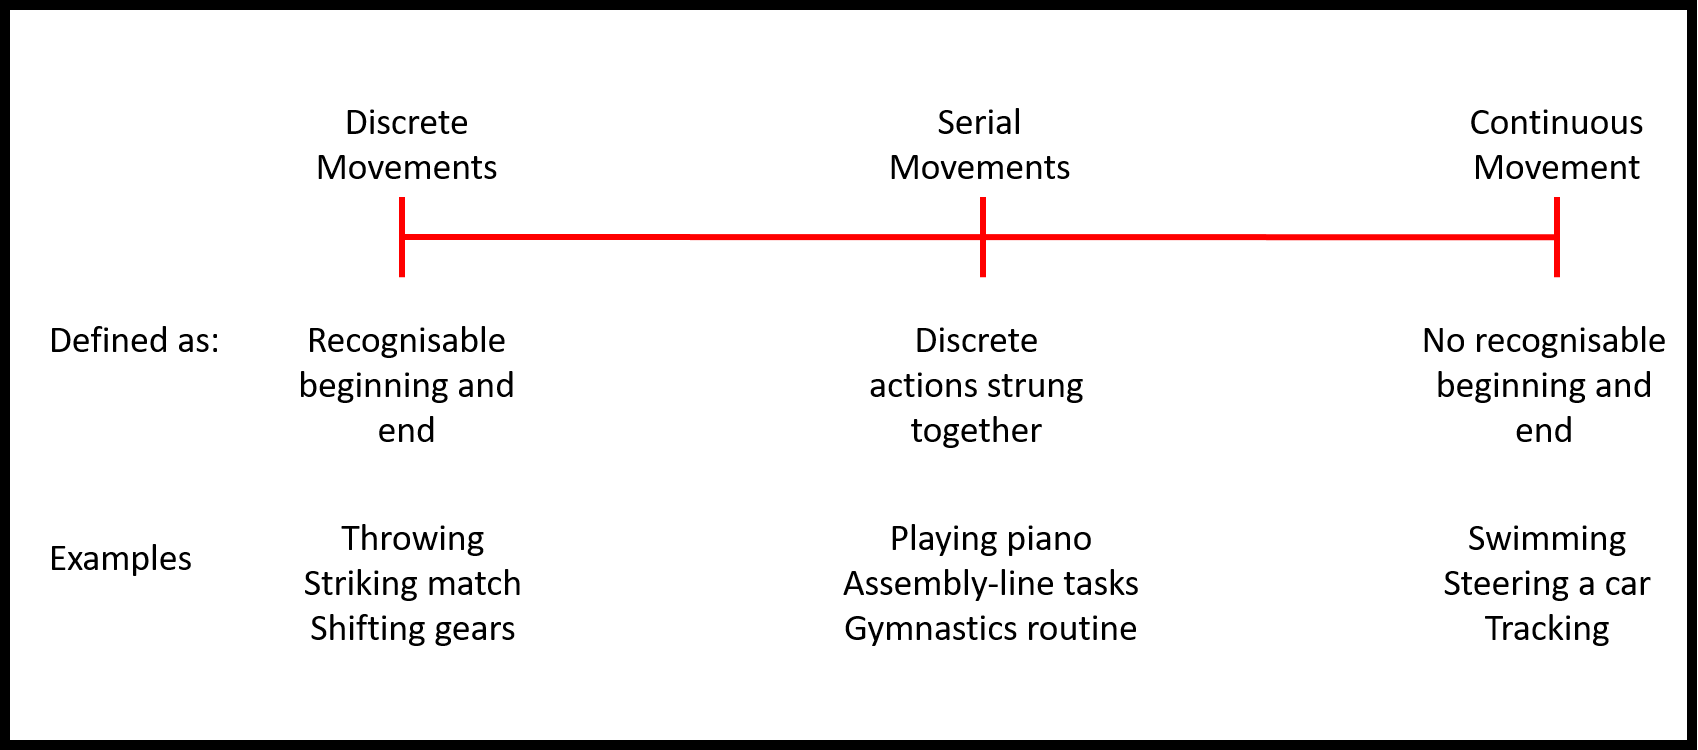
\includegraphics[width=0.49\textwidth]{figures/movement_classification.png}
	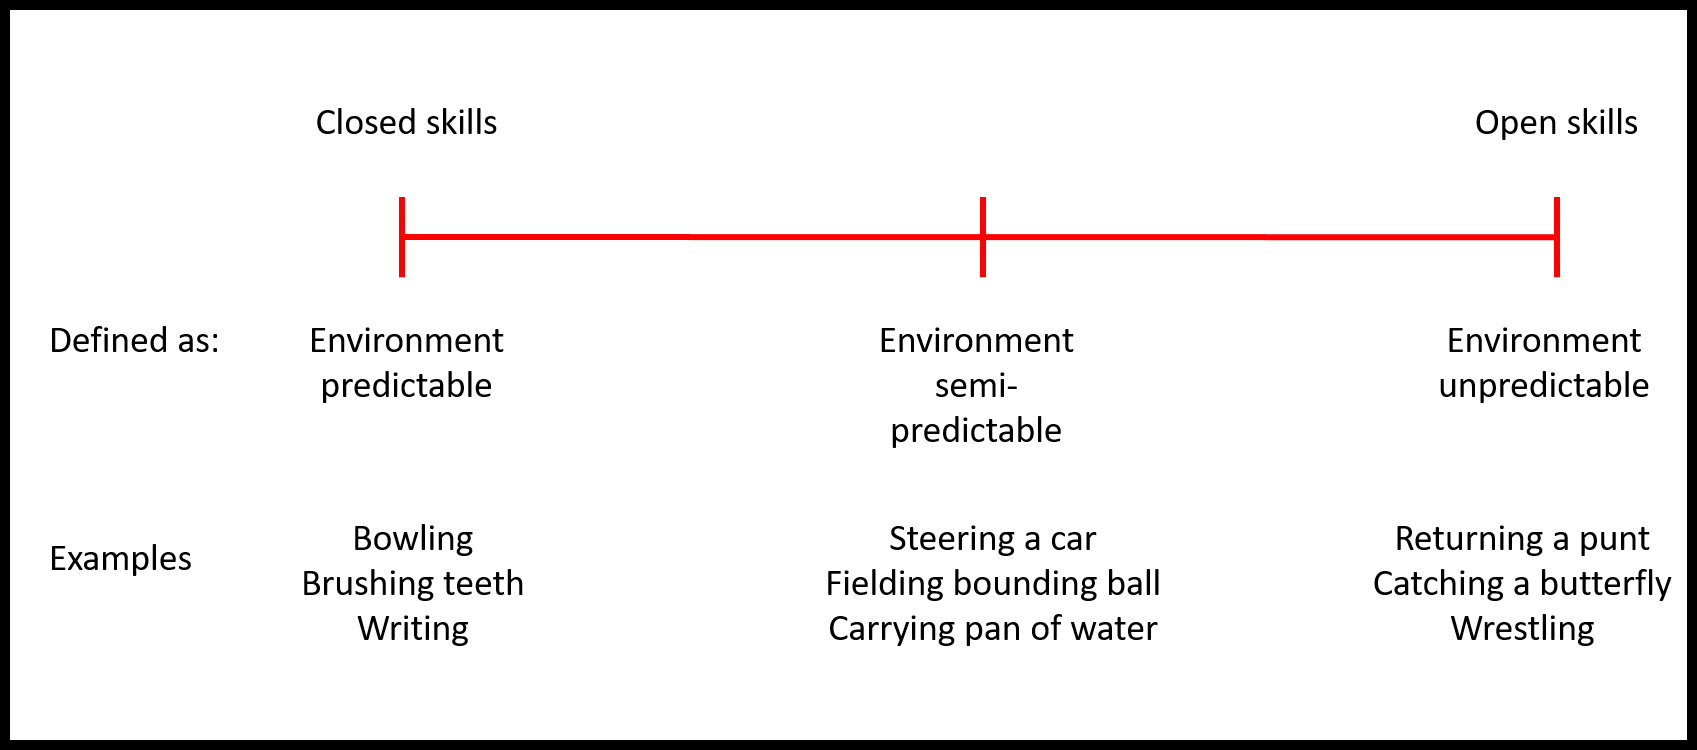
\includegraphics[width=0.49\textwidth]{figures/movement_classification2.png}
	\caption[Movement classifications by Scmidt et al.]{Movement classification by \textit{particualar movements} (left) and \textit{perceptual attributes} by Smift at al.~\cite{mlbook}}
	\label{fig:movement_classification}
\end{figure}

\subsection{Measurements for Motor Learning}
\label{section:measures_for_ml}
The movements of a teacher and the movement of a learner differ. To assess the difference between the two movements, two main classes of measures can be applied~\cite{mlbook}: \textit{measures of error for a single object} and \textit{measures of time and speed}.
\textit{Measure of error for a single object} represent the degree to which the target movement is amiss. Schmidt et al.~\cite{mlbook} provide five \textit{error measures} to calculate this error. Among them, \textit{Constant Error} is the most common measure in related work to determine the difference between the movement of the learner and the movement of the teacher, for example~\cite{perspectivematters,thaichichua,YouMove,onebody,vrdancetrainer,lightguide,physioathome}. Constant Error is defined as the average error between the learner's movments and the teachers movement and is described as
\begin{equation}
	\label{eq:constanterror}
	CE=\frac{\sum_i(x_i-T)}{n}
\end{equation}
with $x_i$: actual value, $T$: target value, $n$: number of values~\cite{mlbook}.\\
The basic idea of \textit{measures of time and speed} is that a performer who can accomplish more in a given amount of time or who can accomplish a given amount of behaviours in less time is more skilful. In related work, this measure is mostly assessed by the task completion time, for example~\cite{perspectivematters,onebody,lightguide}.


\section{Visual Perspectives}
\label{section:visual_perspectives}
\begin{figure}[H]
	\centering
	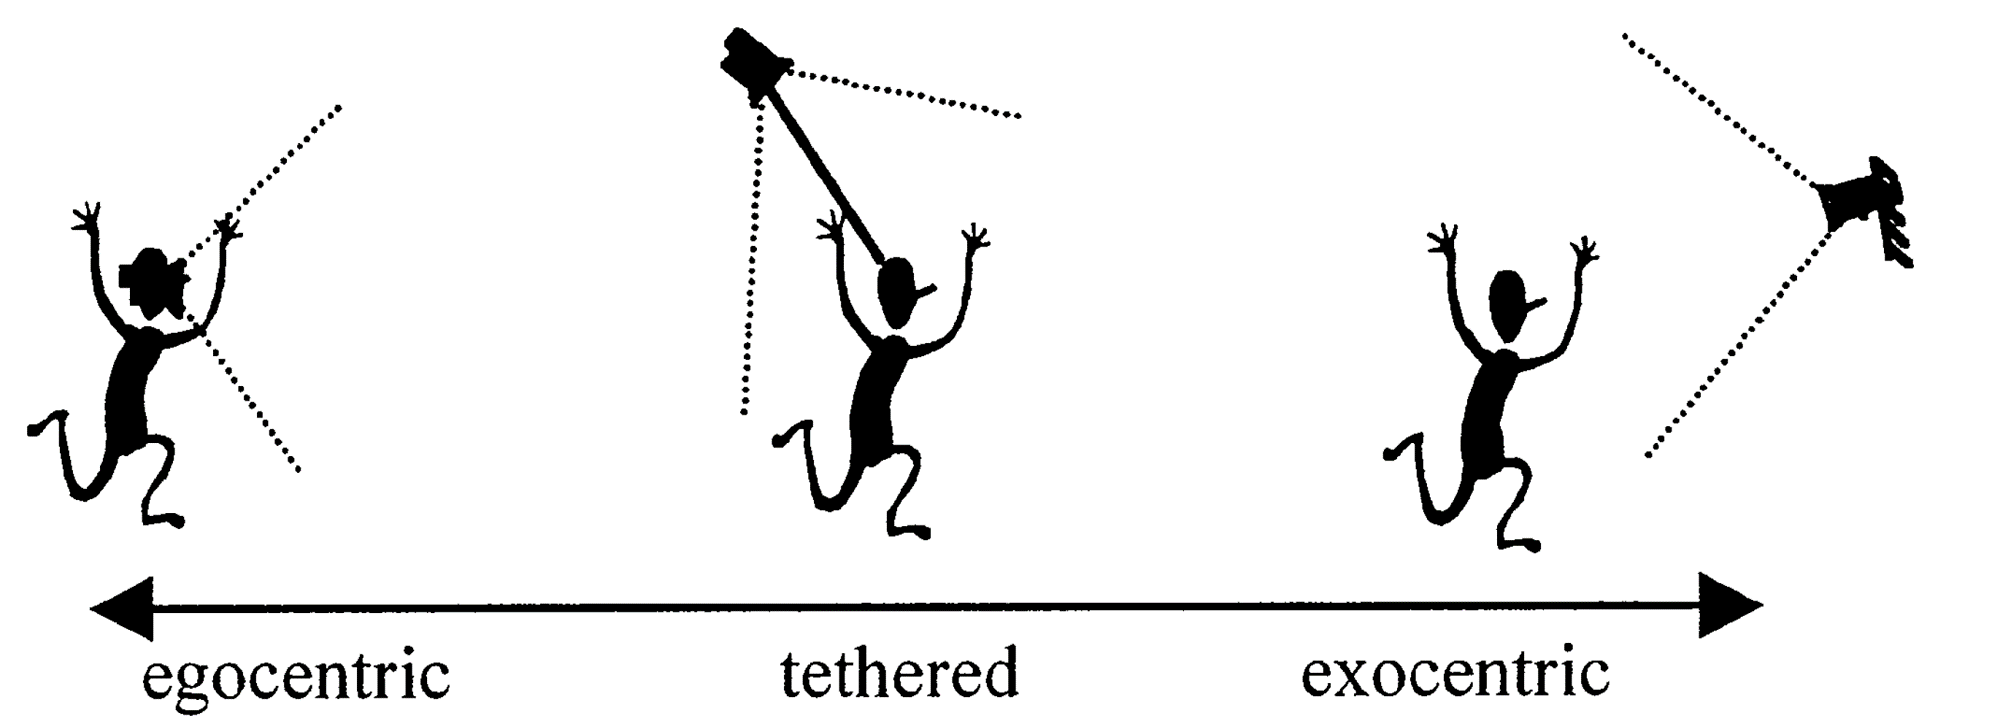
\includegraphics[width=\textwidth]{figures/ego_exo_continuum.PNG}
	\caption[Centricity continuum]{Centricity continuum by Wang and Milgram~\cite{centricitycontinuum}}
	\label{fig:ego-exo-continuum}
\end{figure}
Wang and Milgram~\cite{centricitycontinuum} describe visual perspectives (VP) by the \textit{centricity continuum}, compare figure~\ref{fig:ego-exo-continuum}. On the left extreme on the continuum, the ego-centric VP is located, in literature also called first-person perspective (1PP). On the right extreme, is the exo-centric VP, in literature also called third-person perspective (3PP). The middle part represents tethered VP. By moving from the left to the right, the so-called \textit{tethering distance} increases. The \textit{tethering distance} describes the distance of the anchor point of the eyes to the object in question. In this master's thesis, the "object in question" is the human-shaped guidance visualisation (avatar). VPs can be clustered into three classes: ego-centric VPs (g-class), exo-centric VPs (x-class) and VPs that contain both ego-centric and exo-centric VPs (gx-class). Without the usage of additional perpsective influencing artefacts like mirrors, cameras or screens, there are five possible VPs:
\begin{itemize}
	\item \textbf{Ego-centric}: the teachers avatar is located inside the learners avatar. The learner sees the GV inside the own body, compare figure~\ref{fig:perspectives} top left and figure~\ref{fig:ego}.
	\item \textbf{Purely exo-centric}: the teachers avatar is loacted outside the learners avatar. The learner sees the GV, e.g. in front of him/her, compare figure~\ref{fig:perspectives} top middle.
	\item \textbf{Augmented exo-centric}: the teachers avatar is located outside the learners avatar. Additionally, a virtual copy of the learners avatar is located inside the teachers avatar, compare figure~\ref{fig:perspectives} bottom middle and figure~\ref{fig:exo}.
	\item \textbf{Purely ego \& exo-centric}: the combination of purely ego-centric VP and purely exo-centric VP. The learner sees the GV as well as inside and outside of the own body, compare figure~\ref{fig:perspectives} top right.
	\item \textbf{Ego \& augmented exo-centric}: the combination of the ego-centric VP and the augmented exo-centric VP; the learner sees the GV inside the own body, as well as outside. Additionally, a virtual copy of the learner is located inside the exo-centric GV, compare figure~\ref{fig:perspectives} bottom right and figure~\ref{fig:egoexo}.	
\end{itemize}
\begin{figure}[htb]
	\centering
	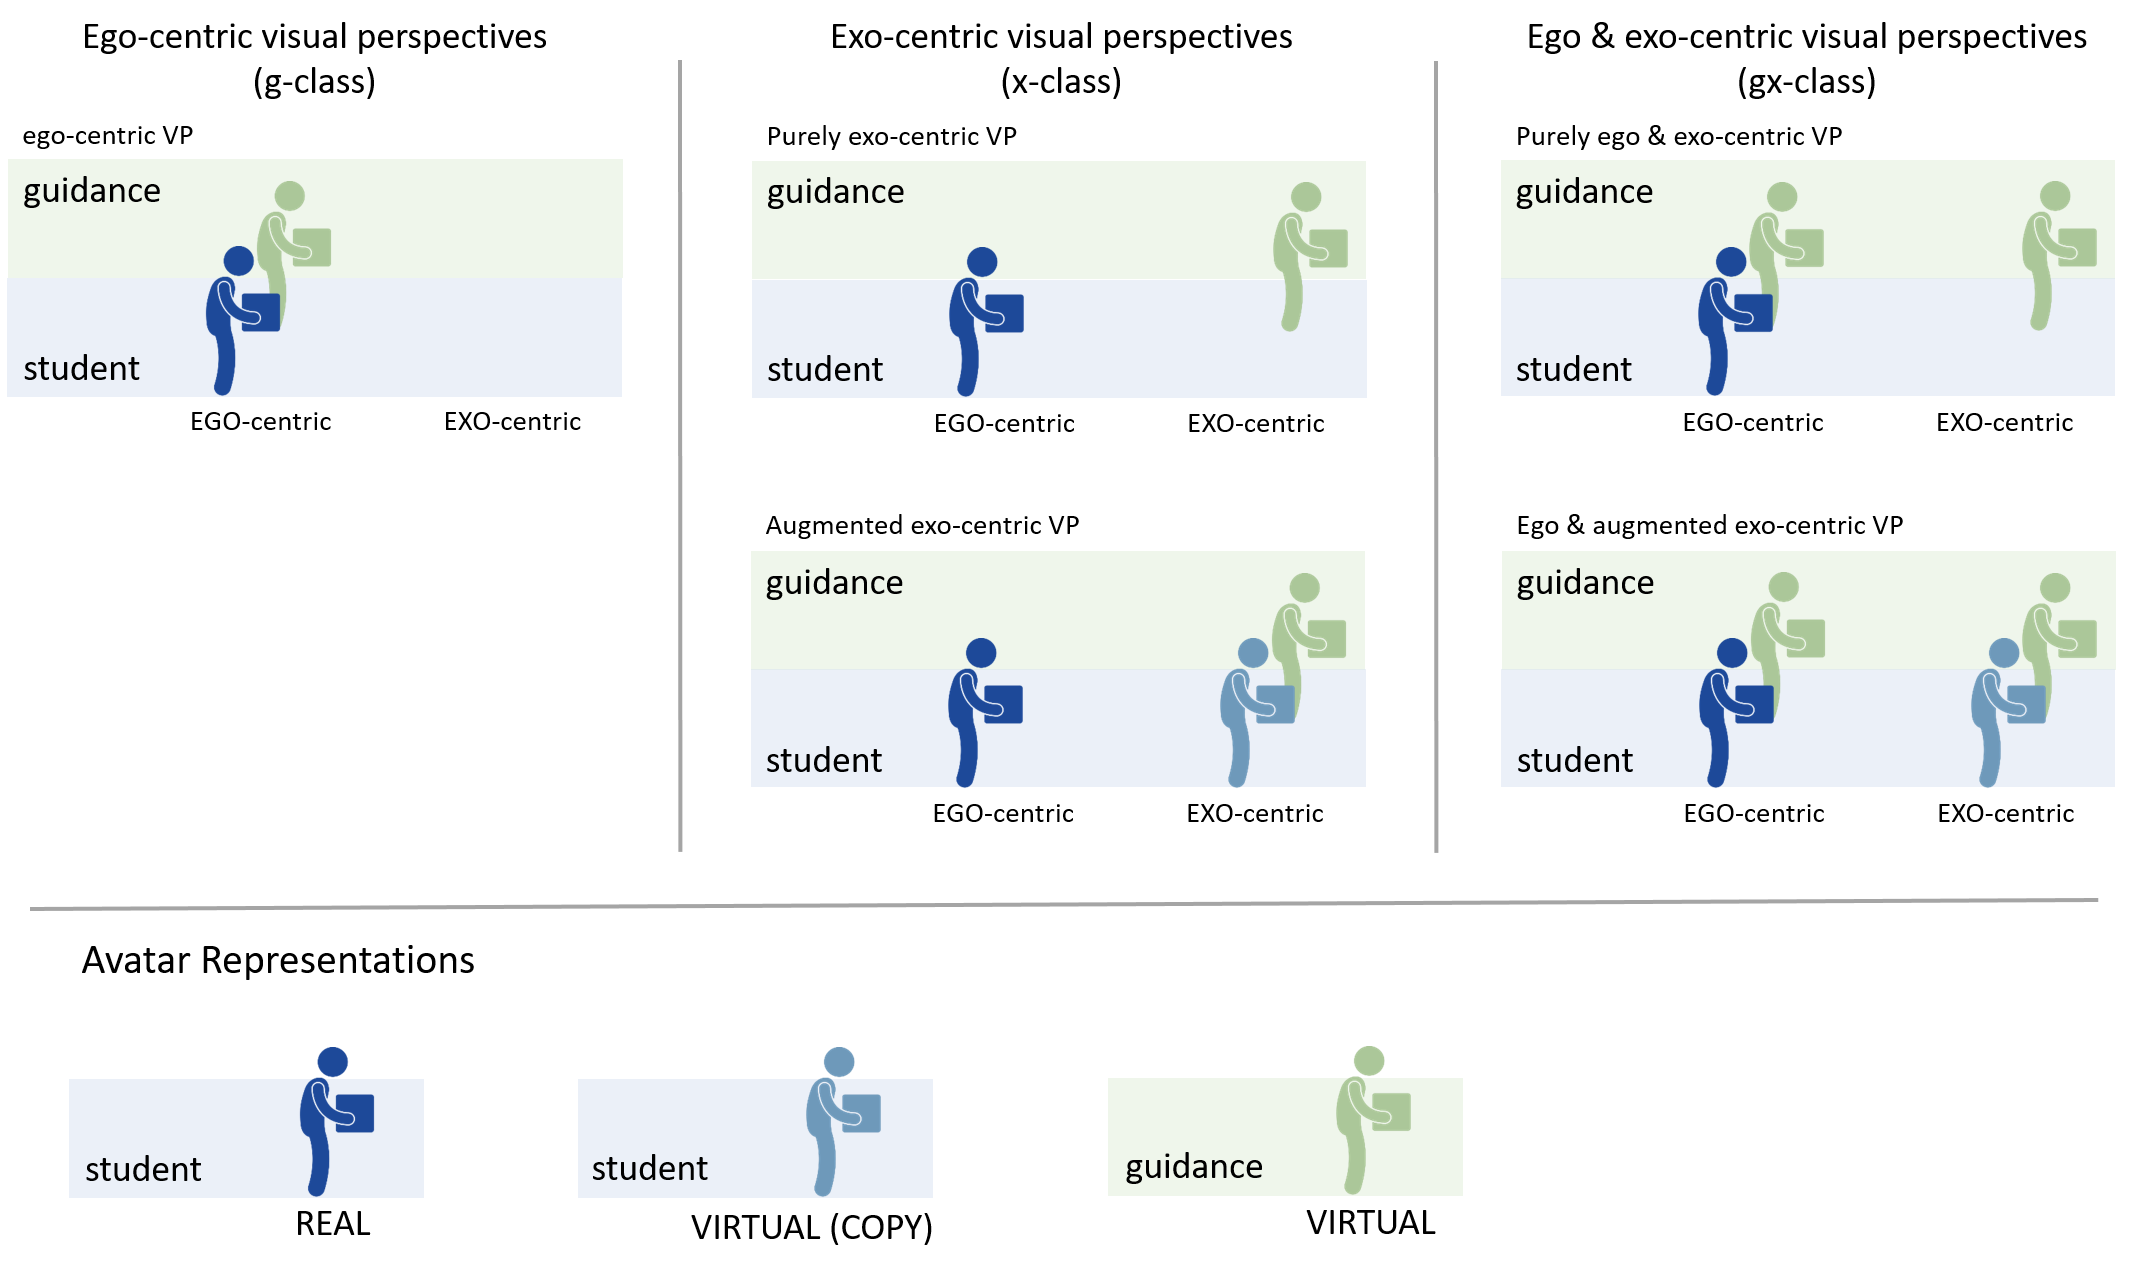
\includegraphics[width=\textwidth]{figures/perspectives_new.png}
	\caption[Visual perspectives]{Visual perspectives clustered by their corresponding class.}
	\label{fig:perspectives}
\end{figure}

\section{Handling Physical Load}
\label{section:handlingphysicalload}
Handling physical load is part of the more general topic Manual Material Handling (MMH). MMH is composed of five elemental tasks: lift, lower, push, pull and hold~\cite{mmh}. Additionally, there are non-elemental tasks like turning and sliding (ibid.). This master's thesis will use a study tasks that include the handling of physical load. Evidently, the task should consist of these elemental tasks. A task that consists of elemental tasks can be generalised to other tasks to a certain extend. To gain a stronger data basis, multiple elemental tasks can be chained together and repeated, to form a so-called Unit-Combined-MMH, ibid.. In chapter~\ref{sec:taskDesign} is described how the elemantal tasks become sub-tasks of the study task.\todo{task motivieren}

\section{Injury Risk Metrics}
\label{section:rm}
Muckell et al.~\cite{muckell} identifyed four main features which are common in the bio-mechanical evaluation of different lifting and carrying techniques. Based on those four features, they defined four injury risk metrics to define low risk and high risk movements.  The four risk metrics (RM) are described in the following. \textit{Support base} describes the distance between the feet. With a proper support base, an individual is more stable while performing a movent like lifting or lowering. \textit{Squat} describes the distance between pelvis and floor. "A proper \textit{squat} reduces injury risk, since the lifting force is applied useing legs and not the back" (ibid.). \textit{Upright stance} is defined by the angle between the upright vector and the bend of the back of an individual. \textit{Spine twist} is the angle between the lines between the left and right shoudler and the left and right hip.

\section{Related Work: Motor Learning in Virtual Reality}
\label{section:related_work}
\begin{table}[H]
	\begin{tabularx}\textwidth{@{}XXXX@{}}
		\toprule
		g-class & x-class & g-class and x-class & gx-class \\ \midrule
		AR-Arm \cite{ararm} & MotionMA \cite{motionma} & OneBody \cite{onebody} & Tai Chi Trainer \cite{thaichichua} \\
		Just Follow Me \cite{justfollowme} & YouMove \cite{YouMove} & LightGuide \cite{lightguide} & SleeveAR \cite{sleevear} \\
		Ghostman \cite{ghostman} & VR Dance Trainer \cite{vrdancetrainer} & MR Dance Trainer \cite{mrdancetrainer} & \\
		Stylo Handifact \cite{stylo} & Physio@Home \cite{physioathome} & Throw Simulator \cite{freethrowsimulator} & \\
		GhostHands \cite{ghosthands} & OutsideMe \cite{outsideme} & Training Phys. Skill \cite{trainingphysicalskills} & \\
		& E-Learning MA \cite{elearningma} &  &  \\
		& My Tai Chi \cite{mythaichicoaches}  & &\\
		& Perform. Training \cite{performancetraining} & &\\
		& RT Gestrue Recognition \cite{rtgesturerecognistion} & &\\
		& KinoHaptics \cite{kinohaptics} & &\\
		& TIKL \cite{tikl} & &\\ \bottomrule
	\end{tabularx}
	\caption[Overview seminar evaluation]{Overview of related work divided by perspective and task}
	\label{tab:rw_overview}
\end{table}

Training movements in Virtual Reality were investigated previously in several works. An overview differentiated by the VP the reasearchers used to train movements is provided in~\ref{tab:rw_overview}. AR-Arm~\cite{ararm}, Just Follow Me~\cite{justfollowme}, Ghostman~\cite{ghostman}, Stylo and Handifact~\cite{stylo} and GhostHands~\cite{ghosthands} used the ego-centric VP. MotionMA~\cite{motionma}, YouMove~\cite{YouMove}, VR Dance Trainer~\cite{vrdancetrainer}, Physio@Home~\cite{physioathome}, OutsideMe~\cite{outsideme}, E-learning Martial Arts~\cite{elearningma}, My Tai-Chi coaches~\cite{mythaichicoaches}, Performance Training~\cite{performancetraining}, Real Time Gesture Recognition~\cite{rtgesturerecognistion}, KinoHaptics~\cite{kinohaptics} and TIKL~\cite{tikl} used a VP from the g-class. There are also works that used to train movements in g-class and x-class, like OneBody~\cite{onebody}, LightGuide~\cite{lightguide}, Mixed Reality Dance Trainer~\cite{mrdancetrainer}, Free Throw Simulator~\cite{freethrowsimulator} and Training Physical Skills~\cite{trainingphysicalskills}. It is little research done for movement training in the gx-class, for example Tai Chi Trainer~\cite{thaichichua} and SleeveAR~\cite{sleevear}.\\
The task which the refferred works use araise from the fields of dancing~\cite{YouMove,vrdancetrainer,outsideme,performancetraining,mrdancetrainer}, sports~\cite{freethrowsimulator,trainingphysicalskills}, rehabilitation~\cite{motionma,physioathome,kinohaptics,sleevear,veimprovesml}, arts~\cite{ararm,justfollowme,stylo,elearningma,mythaichicoaches,rtgesturerecognistion,onebody,thaichichua} and others~\cite{tikl,lightguide}. None of them include the ergonomic handling of a physical load, but sometimes include physical artefacts like a ball (e.g. Free Throw Simulator~\cite{}) or chop sticks (Ghostman~\cite{ghostman}). Also none include locomotional movements.\\
The body parts that are included in the above mentioned task vary, too. For example, \cite{YouMove, thaichichua,onebody,vrdancetrainer} full body movements are taken into consideration, while \cite{ararm,sleevear,ghosthands} uses arm movements.\\
The guidance visualisations which are used to train movements are stick figures~\cite{onebody,YouMove,vrdancetrainer,performancetraining}, wireframes\cite{thaichichua,mrdancetrainer}, human-shaped avatars\cite{thaichichua,vrdancetrainer,trainingphysicalskills,mythaichicoaches} and indicators~\cite{ararm,physioathome,sleevear,ghostman}.\\
To determine to what extend the movements of the learner matcher the GV, different measures are applied. Most common are performance measures based on the accuracy of the performend movements (e.g.~\cite{YouMove,thaichichua,vrdancetrainer,onebody,lightguide,physioathome}) and the time related measurements like the task completion time (e.g.~\cite{lightguide,onebody}).\\
How the perspective influences the learners performance is sparsely investigated. Recently, in December 2020, Yu et al.~\cite{perspectivematters} conducted three independent studies to close this gap. In the first study, Yu et al. compared the ego-centric visual perspective and a 2D-mirror for single arm movements. In the second study, they compared the ego-centric and exo-centric visual perspective for Yoga. In the third study, they compared the ego-centric visual perspective with a 3D-mirror for arm movements. Yu et al. conclude their findings in a design guideline for systems training Motor Learning in Virtual Reality: use the ego-centric visual perspective if the type of motion allows, consider alternatives for other types of motions, ibidem. In all three studies, the ego-centric visual perspective outperformed the other perspectives if the movement was completely visible from the ego-centric visual perspective. \cite{onebody,lightguide} compared their ego-centric VP with their exo-centric VP and for the task they used, the ego-centric VP outperformed the exo-centric VP. \cite{YouMove,vrdancetrainer} compared the movment learning in VR with traditional video based movement learning. In both cases, VR movement learning outperformed video movement learning.\\

\subsection{Research Contribution Statement}
\label{sec:delimination_contribution}
As depicted in the last section, Motor Learning in the gx-class VPs is rarely investigated. Furthermore, Motor Learning that includes the handling of a physical load in VR in different VPs was not part of investigations. Additionally, previous works used stationary task in the ego-centric VP.\\
The proposed experiment in this master's thesis will provide an empirical contribution by increasing the empicial evidence of how the VP influences Motor Learning by guiding full body movements in three VP: ego-centric, exo-centric and the pure combination of them. Furthermore, empirical evidence is generated for Motor Learning including the handling of a physical load. An artifact contribution is provided by presenting a method for guiding locomotion movements in the ego-centric VP.\\

The generated data of the proposed experiment will help designers of VR Motor Learning systems to choose a reasonable perspective for their project.


%The preceding seminar thesis provided an overview over 23 (compare table~\ref{tab:rw_overview}) of these works and evaluated six of them in detail: Tai Chi Trainer by Chua et al.~\cite{thaichichua}, YouMove by Anderson et al.~\cite{YouMove}, VR Dance Trainer by Chan et al.~\cite{vrdancetrainer}, OneBody by Hoang et al.~\cite{onebody}, LightGuide by Sodhi et al.~\cite{lightguide} and Pyhsio@Home by Tang et al.~\cite{physioathome}. Special attention was paid to the VP, task, GV and their independent and dependent variables they used in their investigations. Finally, the results of these works were concluded. An overview is depicted in table~\ref{tab:rw_overview_detail}.

%These works inform this work in various aspects. Chua et al. used the ego \& augmented exo-centric VP, Hoang et al. and Sodhi et al. the ego-centric visual perspective. These visual perspectives proved to be suited for the evaluation of Motor Learning in VR and is adopted for the proposed study design, compare section~\ref{section:visual_perspectives}. Furthermore, Chan et al. and Chua et al. used high realistic avatars as guidance visualisation, which are used in the proposed study design, compare seminar thesis chapter 3.3. Additionally, recent research indicates that high realism avatars outperform abstract avatars~\cite{max,perspectivematters}. All authors used a performance measure to evaluate the performed movements of the participants of their studies. Primarily the distance-based measures informed the measures used in the proposed study design\\%compare figure ??? yxc
%The above mentioned works do not use the relatively new technology of Vive Trackers in combination with Inverse Kinematics (IK, see project report chapter 2.1 and 2.2). Sra et al.~\cite{samesetup} used this technology in 2018 for their system Your Place and Mine to render human-shaped avatars.\\
%The results of related work yielded no clear conclusion about the influence of the perspectives on motor learning. Chua et al. found no difference in the performance between the visual perspectives, Anderson et al. and Chan et al. found out that their exo-centric visual perspectives in Virtual Reality outperform traditional video guidance. Hoang et al. and Sodhi et al. conclude that the ego-centric perspective outperforms the exo-centric visual perspective. Nevertheless, an investigation of how the visual perspective influences motor learning was not investigated.  This work, in contrast, focuses on full-body movements that include the handling of physical load. Furthermore, this work provides a third visual perspective, where the ego-centric and exo-centric visual perspective is combined.

%VR already proved to be a suitable environment for Motor Learning for tasks like dancing~\cite{YouMove,vrdancetrainer,outsideme,performancetraining,mrdancetrainer}, sports~\cite{freethrowsimulator,trainingphysicalskills}, Rehabilitation~\cite{motionma,physioathome,kinohaptics,sleevear,veimprovesml}, arts~\cite{ararm,justfollowme,stylo,elearningma,mythaichicoaches,rtgesturerecognistion,onebody,thaichichua} and others~\cite{tikl,lightguide}.
 



%\todo{new papers occured, read them, then write this statement. notes:}
%what is done:  v
%comparing ego-centric with exo-centric video.
%comparing ego-centric with exo-centric and the combination, but yielded to no result, because old paper and old pc
%comparing with mirrors,
%comparing isolated body parts
%everyone made his live easy by just looking at stationary movements, mostly containing only some body parts.
%new: nobody did fullbody movements with locomotion. ego-centric locomotion motion guidance is completely new. 
%related work only investigated on stationary movements. but motor learning is not stationary. body parts is also not stationary.
%real-world relation poor because of arts dance or abstract. my work is the first one haveing really a task that is reasonable!\\
%Previous work investigated the differences between the perspectives, but:
%To my knowledge, there is no investigation on full body movements that include locomotion. Furthermore, there are on investigations that include the handling of physical load.
%Perivous works compared ego-centric Motor Learning with video learning\cite{YouMove,vrdancetrainer}, augemnted mirrors\cite{perspectivematters,onebody}.
%The conduction of the proposed study will produce data that serves as a reasonable basis for designers of VR Motor Learning systems choosing a suitable perspectives. This is achieved by an Empirical Research Contribution. The empirical data is gathered by a comparative study between the ego-centric visual perspective, the exo-centric visual perspective and the combination. As novelty, the task includes handling of physical load which consists of the elemental tasks of manual material handling. This allows an evaluation of the elemental tasks per visual perspective and can give insights which perspective is suited for specific tasks.\\
%Additionaly, an artifact contribution is provided by the ego-centric guidance of locomotion movements.

%direct comparison not even in tai chi chua
